\documentclass[12pt,a4paper]{report}
\usepackage[utf8]{inputenc}
\usepackage{amsmath,amsfonts,amssymb}
\usepackage{graphicx}
\usepackage{hyperref}
\usepackage{longtable}
\usepackage{geometry}
\usepackage{booktabs}
\usepackage[table]{xcolor}
\usepackage{tikz}
\usetikzlibrary{shapes.geometric, arrows.meta, positioning, fit, calc}
\usepackage{float}
\usepackage{enumitem}
\usepackage{caption}
\usepackage{fancyhdr}
\usepackage{setspace}
\usepackage{titlesec}
\usepackage{subcaption}

\geometry{margin=1in}
\onehalfspacing

\definecolor{headercolor}{RGB}{41,128,185}
\definecolor{lightgray}{RGB}{240,240,240}

\pagestyle{fancy}
\fancyhf{}
\fancyhead[L]{\small Credit Risk Prediction Model}
\fancyhead[R]{\small Fr.\ CRCE}
\fancyfoot[C]{\thepage}

\begin{document}

% ==================== TITLE PAGE ====================
\begin{titlepage}
\centering
\vspace*{1cm}
{\large\textbf{Fr.\ Conceicao Rodrigues College of Engineering, Bandra}\\[0.3cm]}
{\normalsize (Affiliated to University of Mumbai)\\[0.2cm]}
{\normalsize Department of Computer Engineering\\[1.5cm]}
{\Huge\bfseries Credit Risk Prediction Model\\[0.3cm]}
{\Large\bfseries Using Machine Learning with\\Explainable AI\\[1.5cm]}
{\large\textbf{A Mini Project Report}\\[0.2cm]}
{\normalsize Submitted in partial fulfillment of the requirements for the\\
degree of Bachelor of Engineering in Computer Engineering\\[1.5cm]}
{\large\textbf{Submitted by:}\\[0.4cm]}
\begin{tabular}{l l}
1. & Ralph Joseph Dsouza (10242) \\
2. & Chris Fernandes (10244) \\
3. & Ijas Keni (10253) \\
\end{tabular}\\[1.5cm]
{\large\textbf{Under the Guidance of:}\\[0.3cm]}
Prof.\ Sohan Agate\\[1.5cm]
{\large\textbf{Principal:} Dr.\ Sapna Prabhu\\[1cm]}
{\large Academic Year 2025--2026\\}
\end{titlepage}

% ==================== CERTIFICATE ====================
\newpage\thispagestyle{empty}
\begin{center}{\Large\bfseries CERTIFICATE}\\[1cm]\end{center}
This is to certify that the Mini Project entitled \textbf{``Credit Risk Prediction Model Using Machine Learning with Explainable AI''} submitted by:
\begin{enumerate}
\item Ralph Joseph Dsouza (10242)
\item Chris Fernandes (10244)
\item Ijas Keni (10253)
\end{enumerate}
\noindent in partial fulfillment of the requirements for the degree of \textbf{Bachelor of Engineering} in \textbf{Computer Engineering} from the \textbf{University of Mumbai} is a record of bonafide work carried out under my supervision during the academic year 2025--2026.
\vspace{2cm}
\noindent
\begin{tabular}{p{7cm}p{7cm}}
\textbf{Guide:} & \textbf{Principal:} \\[1.5cm]
\rule{5cm}{0.4pt} & \rule{5cm}{0.4pt} \\
Prof.\ Sohan Agate & Dr.\ Sapna Prabhu \\
Dept.\ of Computer Engineering & Fr.\ CRCE, Bandra \\
\end{tabular}
\vspace{2cm}
\noindent\textbf{External Examiner:}\\[1.5cm]
\rule{5cm}{0.4pt}

% ==================== ACKNOWLEDGEMENT ====================
\newpage\thispagestyle{empty}
\begin{center}{\Large\bfseries ACKNOWLEDGEMENT}\\[1cm]\end{center}
We would like to express our sincere gratitude to our project guide, \textbf{Prof.\ Sohan Agate}, for his invaluable guidance, continuous encouragement, and constructive suggestions throughout the development of this project. His expertise in machine learning and data science helped shape the direction of our work significantly.

We are deeply grateful to our Principal, \textbf{Dr.\ Sapna Prabhu}, and the Head of the Department of Computer Engineering for providing us with the necessary infrastructure and academic environment to carry out this project.

We extend our thanks to the faculty members of the Department of Computer Engineering at \textbf{Fr.\ Conceicao Rodrigues College of Engineering, Bandra}, for their support and knowledge sharing during the course of this project.

We also acknowledge the open-source community and the authors of the IEEE research papers referenced in this work, whose published findings provided the academic foundation for the features implemented in our system.

Finally, we thank our families and friends for their constant support and encouragement.
\vspace{1.5cm}
\noindent
\begin{tabular}{l}
Ralph Joseph Dsouza (10242)\\
Chris Fernandes (10244)\\
Ijas Keni (10253)\\
\end{tabular}

% ==================== ABSTRACT ====================
\newpage\thispagestyle{empty}
\begin{center}{\Large\bfseries ABSTRACT}\\[1cm]\end{center}
Credit risk assessment is a critical function in the financial industry, where the ability to accurately predict loan defaults directly impacts a lender's profitability and stability. Traditional credit scoring methods, such as rule-based systems and single-model approaches, often fail to capture the complex, non-linear relationships present in modern borrower data and lack the transparency demanded by evolving regulatory frameworks like the GDPR and RBI Fair Lending Guidelines.

This project presents a comprehensive, end-to-end \textbf{Credit Risk Intelligence Platform} that addresses these limitations by combining a multi-model machine learning ensemble with Explainable AI (XAI). The system trains and compares four classification algorithms---Logistic Regression, XGBoost, LightGBM, and Random Forest---on a credit risk dataset of approximately 50,000 loan applications. To address the inherent class imbalance (a 10\% default rate), SMOTE-Tomek resampling is applied, and Optuna Bayesian optimization is used for automated hyperparameter tuning, resulting in a best-performing model achieving 93\% accuracy, 94\% recall, and an AUC-ROC of approximately 0.99.

The platform is deployed as an interactive Streamlit web application featuring: (i) individual and batch credit risk prediction with real-time credit score generation on a 300--900 scale, (ii) a SHAP-based explainability dashboard that decomposes each prediction into per-feature contributions, (iii) a model performance analytics page with ROC curves, AUC visualizations, precision-recall curves, and confusion matrices, (iv) macroeconomic stress testing to simulate borrower resilience under economic shocks, and (v) an algorithmic fairness audit module.

\vspace{0.5cm}
\noindent\textbf{Keywords:} Credit Risk, Machine Learning, Logistic Regression, XGBoost, LightGBM, Random Forest, SHAP, Explainable AI, SMOTE-Tomek, Optuna, Streamlit.

% ==================== TABLE OF CONTENTS ====================
\newpage
\tableofcontents
\newpage
\listoffigures
\listoftables
\newpage


% ============================================================
%              CHAPTER 1: INTRODUCTION
% ============================================================
\chapter{Introduction}

The global lending industry disburses trillions of dollars annually in consumer and commercial credit. A core challenge facing every lending institution---from multinational banks to peer-to-peer lending platforms---is the accurate assessment of \emph{credit risk}: the probability that a borrower will fail to meet their contractual obligations. Inaccurate risk assessment leads to two costly outcomes: approving loans that eventually default (resulting in direct financial losses) and rejecting creditworthy applicants (resulting in lost revenue and market share).

Traditional credit scoring approaches, such as the FICO score and rule-based expert systems, rely on a small set of hand-crafted rules and linear statistical models. While these methods are interpretable and well-understood by regulators, they struggle to capture the complex, non-linear interactions among dozens of financial, demographic, and behavioural features that characterise modern borrower profiles. Furthermore, real-world credit datasets exhibit severe \emph{class imbalance}---typically only 5--15\% of loan applications result in default---which causes naive classifiers to achieve high accuracy by simply predicting the majority class while failing to identify the very defaulters they are designed to detect.

Recent advances in machine learning---specifically gradient-boosted tree ensembles (XGBoost, LightGBM) and resampling techniques (SMOTE, Tomek Links)---have demonstrated significant improvements in predictive performance on imbalanced credit datasets. Simultaneously, the rise of Explainable AI (XAI) frameworks such as SHAP (SHapley Additive exPlanations) has made it possible to provide transparent, per-feature explanations for individual predictions, satisfying the growing regulatory demand for model interpretability under frameworks such as the GDPR and RBI Fair Lending Guidelines.

This project presents a comprehensive \textbf{Credit Risk Intelligence Platform} that combines multi-model machine learning, SHAP-based explainability, and an interactive Streamlit web interface to deliver an end-to-end credit risk assessment solution. The platform trains four classification algorithms on a dataset of approximately 50,000 loan applications, handles class imbalance via SMOTE-Tomek, optimises hyperparameters with Optuna, and provides a rich set of features including batch prediction, stress testing, fairness auditing, and personalised credit improvement paths.


% ============================================================
%        CHAPTER 2: OBJECTIVES OF THE PROJECT
% ============================================================
\chapter{Objectives of the Project}

The primary objectives of this project are as follows:

\begin{enumerate}[label=\arabic*.]
    \item \textbf{Multi-Model Training and Comparison:} Train and evaluate four classification models---Logistic Regression, XGBoost, LightGBM, and Random Forest---on a credit risk dataset using SMOTE-Tomek resampling for class imbalance and Optuna Bayesian optimisation for automated hyperparameter tuning.

    \item \textbf{High Recall for Default Detection:} Achieve a recall of at least 90\% for the default class while maintaining overall accuracy above 90\%, ensuring that high-risk borrowers are reliably identified. In credit risk, missing a defaulter (false negative) has a far greater cost than incorrectly flagging a non-defaulter (false positive).

    \item \textbf{Explainable AI Integration:} Implement SHAP-based (SHapley Additive exPlanations) explainability to decompose each individual prediction into per-feature contributions. This enables loan officers to understand \emph{why} a borrower received a particular score, satisfying regulatory transparency requirements under GDPR and RBI Fair Lending Guidelines.

    \item \textbf{Interactive Web Application:} Build a production-ready Streamlit web application supporting multiple input workflows: individual manual entry with smart auto-calculated features, preset borrower profiles for quick testing, single-profile CSV upload, and batch CSV upload for processing multiple borrowers simultaneously.

    \item \textbf{Comprehensive Performance Dashboard:} Provide a model performance analytics page with ROC curves (including shaded AUC area visualisation), AUC comparison bar charts, precision-recall curves, confusion matrices, and a fairness audit module---enabling non-technical stakeholders to evaluate model quality.

    \item \textbf{Advanced Risk Assessment Features:} Incorporate macroeconomic stress testing (simulating economic shocks of varying severity), survival analysis (time-to-default probability curves), and personalised credit improvement paths with actionable step-by-step recommendations for low-scoring borrowers.

    \item \textbf{Credit Score Generation:} Map the model's predicted default probability to a standardised credit score on a 300--900 scale with categorical ratings (Poor, Average, Good, Excellent), providing an intuitive output format familiar to industry practitioners.
\end{enumerate}


% ============================================================
%          CHAPTER 3: SCOPE OF THE PROJECT
% ============================================================
\chapter{Scope of the Project}

The scope of this project encompasses the design, development, and local deployment of an end-to-end credit risk assessment platform. The boundaries of the project are defined as follows:

\subsection*{In Scope}
\begin{itemize}
    \item \textbf{Data:} A credit risk dataset of approximately 50,000 loan applications with 24 raw features distributed across three relational tables---customer demographics (\texttt{customers.csv}), loan details (\texttt{loans.csv}), and credit bureau history (\texttt{bureau\_data.csv}). The dataset is sourced from Kaggle and is based on Tunisian commercial bank records.

    \item \textbf{Models:} Four supervised binary classification algorithms---Logistic Regression, XGBoost, LightGBM, and Random Forest---each with automated Optuna hyperparameter tuning (30 Bayesian trials per model) and SMOTE-Tomek resampling for class imbalance.

    \item \textbf{Explainability:} SHAP (SHapley Additive exPlanations) values computed for each prediction, providing per-feature attribution. Pre-computed SHAP explainers are serialised for runtime efficiency.

    \item \textbf{Deployment:} A locally hosted Streamlit web application accessible at \texttt{http://localhost:8501}. The application features three navigable pages: Risk Assessment, Model Performance, and About \& Papers.

    \item \textbf{Prediction Workflows:} Individual prediction via manual form entry or preset profiles, single-profile CSV upload, and batch CSV upload with downloadable results.

    \item \textbf{Advanced Features:} Macroeconomic stress testing (mild, moderate, severe shocks), survival analysis curves, personalised credit improvement paths, and algorithmic fairness auditing (disparate impact analysis across age and residence-type demographics).

    \item \textbf{Visualisation:} Interactive Plotly charts including gauge-style credit score displays, SHAP bar charts, ROC curves with shaded AUC, AUC comparison bar charts, precision-recall curves, and confusion matrix heatmaps.
\end{itemize}

\subsection*{Out of Scope}
\begin{itemize}
    \item Cloud deployment (AWS, GCP, Azure) and auto-scaling infrastructure.
    \item REST API development for third-party system integration.
    \item Real-time data feeds from live banking or credit bureau systems.
    \item Deep learning approaches (neural networks, transformers).
    \item Continuous model monitoring, drift detection, and automated retraining pipelines.
    \item Mobile application development.
\end{itemize}


% ============================================================
%        CHAPTER 4: REVIEW OF LITERATURE
% ============================================================
\chapter{Review of Literature}

Credit risk prediction has been a subject of extensive academic and industrial research. This chapter surveys the most relevant recent works, identifies their contributions and limitations, and explains how the present project addresses the identified gaps.

\section{Survey of Existing Systems}

Table~\ref{tab:litreview} summarises the key existing systems, the algorithms they employ, their contributions, and the gaps they leave unaddressed.

\begin{longtable}{|p{0.6cm}|p{2.5cm}|p{2.3cm}|p{2.3cm}|p{2cm}|p{2.5cm}|}
\caption{Literature Review --- Comparison of Existing Credit Risk Systems}\label{tab:litreview}\\
\hline
\rowcolor{headercolor}
\color{white}\textbf{Sr.} & \color{white}\textbf{Paper / System} & \color{white}\textbf{Algorithms Used} & \color{white}\textbf{Summary} & \color{white}\textbf{Justification} & \color{white}\textbf{Gaps Identified}\\
\hline
\endfirsthead
\hline
\rowcolor{headercolor}
\color{white}\textbf{Sr.} & \color{white}\textbf{Paper / System} & \color{white}\textbf{Algorithms Used} & \color{white}\textbf{Summary} & \color{white}\textbf{Justification} & \color{white}\textbf{Gaps Identified}\\
\hline
\endhead

1 & Effective Credit Risk Prediction Using Ensemble Classifiers~\cite{paper1} & RF, AdaBoost, XGBoost, LightGBM, SMOTE-ENN & Multi-model ensemble with SHAP for interpretability & Shows ensemble outperforms single models & No interactive deployment; no batch processing \\
\hline
2 & Explainability of ML Scoring in P2P Lending~\cite{paper2} & Gradient Boosting, SHAP & SHAP analysis of feature-target relationships in lending & Regulatory-grade transparency & Limited to single model; no user-facing dashboard \\
\hline
3 & Credit Risk Assessment using Ensemble Models \& XAI~\cite{paper3} & CatBoost, XGBoost, LightGBM & Achieves AUC-ROC of 0.9693 with XAI compliance & Regulatory compliance focus & No stress testing; no fairness audit \\
\hline
4 & Credit Risk Prediction Based on ML Methods~\cite{paper4} & XGBoost, Logistic Regression & Feature engineering comparison for credit risk & Shows importance of derived features & No automated feature calculation for end users \\
\hline
5 & Incremental Learning Ensemble for Imbalanced Credit~\cite{paper5} & Incremental Ensemble, SMOTE & Batch processing for continuous incoming data & Handles data drift and imbalance & No interactive UI; no explainability layer \\
\hline
6 & Traditional FICO Score System & Linear Regression, Rule-based & Industry-standard 300--850 credit score & Widely adopted and understood & Cannot capture non-linear patterns; opaque rules \\
\hline
7 & Kaggle Credit Risk Notebooks & Various (LR, RF, XGB) & Community-driven EDA and model comparisons & Open-source benchmarks & No deployment; no explainability; no production UI \\
\hline
8 & Commercial Tools (Experian, CIBIL) & Proprietary & Proprietary scoring models used by bureaus & Industry standard & Closed-source; no transparency; expensive licensing \\
\hline
\end{longtable}

\section{Identified Gaps and How This Project Addresses Them}

Based on the comprehensive survey above, the following key gaps are identified in the existing body of work:

\begin{enumerate}[label=\textbf{Gap \arabic*:}]
    \item \textbf{Lack of End-to-End Deployment.} Most academic studies stop at model evaluation in a Jupyter notebook. They do not provide an interactive, user-facing application that a loan officer or borrower can use directly.

    \textit{Our Solution:} We deploy the entire pipeline as a Streamlit web application with an intuitive UI featuring manual entry, preset profiles, and batch CSV upload with downloadable results.

    \item \textbf{Missing Explainability in Production Systems.} Commercial credit scoring tools (FICO, CIBIL) are opaque, and most research prototypes do not integrate SHAP into a live dashboard.

    \textit{Our Solution:} Every individual prediction is accompanied by a SHAP bar chart that decomposes the result into per-feature contributions, directly embedded in the Streamlit UI.

    \item \textbf{No Stress Testing or Fairness Auditing.} None of the surveyed systems simulate macroeconomic shocks or audit model decisions for demographic bias.

    \textit{Our Solution:} We implement a stress-test simulator and a fairness audit module computing disparate impact ratios across age and housing demographics.

    \item \textbf{No Batch Processing with Actionable Recourse.} Existing batch systems produce scores but do not generate personalised improvement plans for low-scoring borrowers.

    \textit{Our Solution:} Our batch prediction module generates per-borrower improvement paths with specific action items, projected score targets, and approval timelines.

    \item \textbf{Limited Model Comparison Dashboards.} Research papers compare models in tables but rarely provide interactive visualisations accessible to non-technical stakeholders.

    \textit{Our Solution:} A dedicated Model Performance page provides full-width ROC curves with shaded AUC areas, an AUC bar chart, precision-recall curves, and per-model confusion matrices.
\end{enumerate}


% ============================================================
%        CHAPTER 5: PROPOSED SYSTEM
% ============================================================
\chapter{Proposed System}

\section{Drawbacks of Existing System}

The existing credit risk assessment systems---both academic prototypes and commercial products---suffer from several critical drawbacks:

\begin{enumerate}
    \item \textbf{Opaque Decision-Making:} Commercial scoring systems (FICO, CIBIL, Experian) use proprietary, black-box algorithms. Borrowers and loan officers cannot understand \emph{why} a particular score was assigned, making it difficult to contest decisions or identify areas for improvement.

    \item \textbf{Single-Model Limitations:} Most existing systems rely on a single model (typically logistic regression or a single tree-based model). This provides no basis for model comparison and cannot identify whether a different algorithm would yield better performance on the specific data distribution.

    \item \textbf{No Class Imbalance Handling:} Many existing systems train on raw, imbalanced datasets where defaults constitute only 5--15\% of records. This causes models to achieve misleadingly high accuracy by predicting the majority class (non-default), while failing to identify actual defaulters.

    \item \textbf{No Interactive Deployment:} The vast majority of academic credit risk research stops at Jupyter notebook evaluation. There is no production-ready interface that a loan officer can use in practice to enter borrower details and receive predictions in real time.

    \item \textbf{No Stress Testing or Fairness Auditing:} Existing systems do not simulate how predictions would change under adverse economic conditions (inflation, recession) and do not audit whether the model exhibits bias across demographic groups.

    \item \textbf{No Actionable Recourse:} When a borrower is rejected or receives a low score, existing systems provide no guidance on what specific actions the borrower could take to improve their creditworthiness.
\end{enumerate}

\section{Problem Statement}

To design and develop an end-to-end machine learning platform that accurately predicts the probability of loan default, generates a credit score on a 300--900 scale, and provides transparent, SHAP-based explanations for each prediction---while handling class imbalance through SMOTE-Tomek resampling, optimising model hyperparameters via Optuna Bayesian search, and supporting both individual and batch assessment workflows through an interactive Streamlit web interface. The system must also incorporate macroeconomic stress testing, algorithmic fairness auditing, and personalised credit improvement paths to address the gaps identified in existing literature.


% ============================================================
%          CHAPTER 6: SYSTEM DESIGN
% ============================================================
\chapter{System Design}

\section{Block Diagram}

Figure~\ref{fig:arch} presents the layered block diagram of the Credit Risk Intelligence Platform. The system is organised into four horizontal layers: the Presentation Layer (Streamlit frontend), the Application Logic Layer (prediction engine and explainability module), the Model Layer (four trained classifiers and SHAP explainers), and the Data/Artifact Layer (serialised model files, scaler, and metrics).

\begin{figure}[H]
\centering
\resizebox{\textwidth}{!}{%
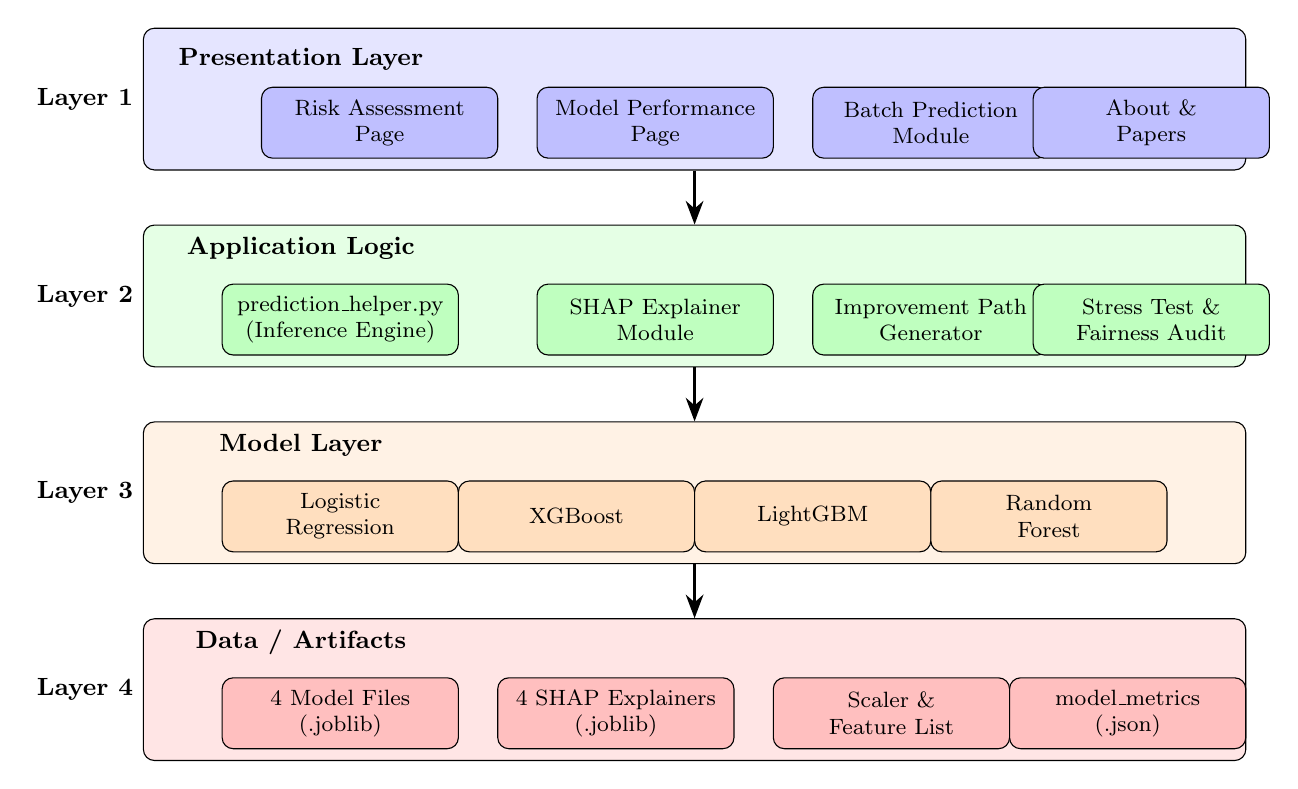
\begin{tikzpicture}[
    layer/.style={draw, rounded corners, minimum width=14cm, minimum height=1.8cm, fill=#1!10, font=\small},
    block/.style={draw, rounded corners, minimum width=3cm, minimum height=0.9cm, fill=#1!25, font=\footnotesize, align=center},
    arrow/.style={-{Stealth[length=3mm]}, thick},
]
% Layer 1 - Presentation
\node[layer=blue, label={[font=\bfseries\small]left:Layer 1}] (L1) at (0,9) {};
\node[font=\bfseries\small] at (-5,9.5) {Presentation Layer};
\node[block=blue] at (-4,8.7) {Risk Assessment\\Page};
\node[block=blue] at (-0.5,8.7) {Model Performance\\Page};
\node[block=blue] at (3,8.7) {Batch Prediction\\Module};
\node[block=blue] at (5.8,8.7) {About \&\\Papers};
% Layer 2 - Application Logic
\node[layer=green, label={[font=\bfseries\small]left:Layer 2}] (L2) at (0,6.5) {};
\node[font=\bfseries\small] at (-5,7.1) {Application Logic};
\node[block=green] at (-4.5,6.2) {prediction\_helper.py\\(Inference Engine)};
\node[block=green] at (-0.5,6.2) {SHAP Explainer\\Module};
\node[block=green] at (3,6.2) {Improvement Path\\Generator};
\node[block=green] at (5.8,6.2) {Stress Test \&\\Fairness Audit};
% Layer 3 - Model Layer
\node[layer=orange, label={[font=\bfseries\small]left:Layer 3}] (L3) at (0,4) {};
\node[font=\bfseries\small] at (-5,4.6) {Model Layer};
\node[block=orange] at (-4.5,3.7) {Logistic\\Regression};
\node[block=orange] at (-1.5,3.7) {XGBoost};
\node[block=orange] at (1.5,3.7) {LightGBM};
\node[block=orange] at (4.5,3.7) {Random\\Forest};
% Layer 4 - Data/Artifact
\node[layer=red, label={[font=\bfseries\small]left:Layer 4}] (L4) at (0,1.5) {};
\node[font=\bfseries\small] at (-5,2.1) {Data / Artifacts};
\node[block=red] at (-4.5,1.2) {4 Model Files\\(.joblib)};
\node[block=red] at (-1,1.2) {4 SHAP Explainers\\(.joblib)};
\node[block=red] at (2.5,1.2) {Scaler \&\\Feature List};
\node[block=red] at (5.5,1.2) {model\_metrics\\(.json)};
% Arrows
\draw[arrow] (L1) -- (L2);
\draw[arrow] (L2) -- (L3);
\draw[arrow] (L3) -- (L4);
\end{tikzpicture}
}
\caption{Block Diagram --- Layered Architecture of Credit Risk Intelligence Platform}
\label{fig:arch}
\end{figure}

\section{Module Description}

\subsection{Algorithms}

\subsubsection{Theoretical Analysis}

The credit risk prediction problem is formulated as a \textbf{supervised binary classification} task. Given a feature vector $\mathbf{x} \in \mathbb{R}^{14}$ representing a borrower's profile, the goal is to predict a binary label $y \in \{0, 1\}$, where $y = 1$ indicates default. The model outputs a probability $P(y=1|\mathbf{x})$ which is mapped to a credit score via $\text{Score} = 300 + 600 \times (1 - P(y=1|\mathbf{x}))$.

The key theoretical challenges addressed are:
\begin{itemize}
    \item \textbf{Class Imbalance:} With only 10\% defaults, the prior probability $P(y=1) = 0.10$. Standard maximum-likelihood training biases models toward the majority class. SMOTE-Tomek resampling balances the training distribution to approximately $P(y=1) \approx 0.50$.
    \item \textbf{Hyperparameter Sensitivity:} Each model family has a distinct set of hyperparameters (e.g., regularisation strength $C$ for LR, tree depth for XGBoost). Optuna uses a Tree-structured Parzen Estimator (TPE) for efficient Bayesian search over these spaces.
    \item \textbf{Explainability:} SHAP values are rooted in cooperative game theory. For a prediction $f(\mathbf{x})$, the SHAP value $\phi_i$ for feature $i$ satisfies: $f(\mathbf{x}) = \mathbb{E}[f(\mathbf{X})] + \sum_{i=1}^{p} \phi_i$, ensuring additive, fair attribution.
\end{itemize}

\subsubsection{Algorithms Used}

\begin{enumerate}
    \item \textbf{Logistic Regression:} Models $P(y=1|\mathbf{x}) = \sigma(\mathbf{w}^T\mathbf{x} + b)$ where $\sigma$ is the sigmoid function. Regularised with L2 penalty (strength $C$ tuned by Optuna). Selected as the best model due to interpretability and highest AUC-ROC (0.9963).

    \item \textbf{XGBoost (eXtreme Gradient Boosting):} Sequentially builds decision trees where each tree corrects the residual errors of the ensemble. Uses gradient descent in function space with $L_1$ and $L_2$ regularisation on leaf weights. AUC-ROC: 0.9938.

    \item \textbf{LightGBM (Light Gradient Boosting Machine):} Uses histogram-based splitting and leaf-wise (best-first) tree growth for faster training on large datasets. Employs Gradient-based One-Side Sampling (GOSS) for efficiency. AUC-ROC: 0.9941.

    \item \textbf{Random Forest:} An ensemble of $n$ independently trained decision trees using bootstrap aggregation (bagging). Each tree is trained on a random subset of features, reducing variance through decorrelation. AUC-ROC: 0.9910.
\end{enumerate}

\subsection{Database(s)}

The project uses a file-based data architecture (no relational database server is required):

\begin{itemize}
    \item \textbf{Input Data:} Three CSV files---\texttt{customers.csv} (demographics), \texttt{loans.csv} (loan details with target variable), \texttt{bureau\_data.csv} (credit bureau history)---merged on \texttt{cust\_id} into a single DataFrame.
    \item \textbf{Model Artifacts:} Trained models (\texttt{.joblib}), SHAP explainers (\texttt{.joblib}), fitted scaler (\texttt{.joblib}), and performance metrics (\texttt{.json}) stored in the \texttt{artifacts/} directory.
    \item \textbf{Runtime State:} Streamlit's \texttt{st.session\_state} dictionary manages user inputs and prediction results in-memory.
\end{itemize}

\subsection{UML Diagram(s)}

Figure~\ref{fig:uml} shows the use-case diagram capturing interactions between the two primary actors and the system's functional use cases.

\begin{figure}[H]
\centering
\resizebox{0.85\textwidth}{!}{%
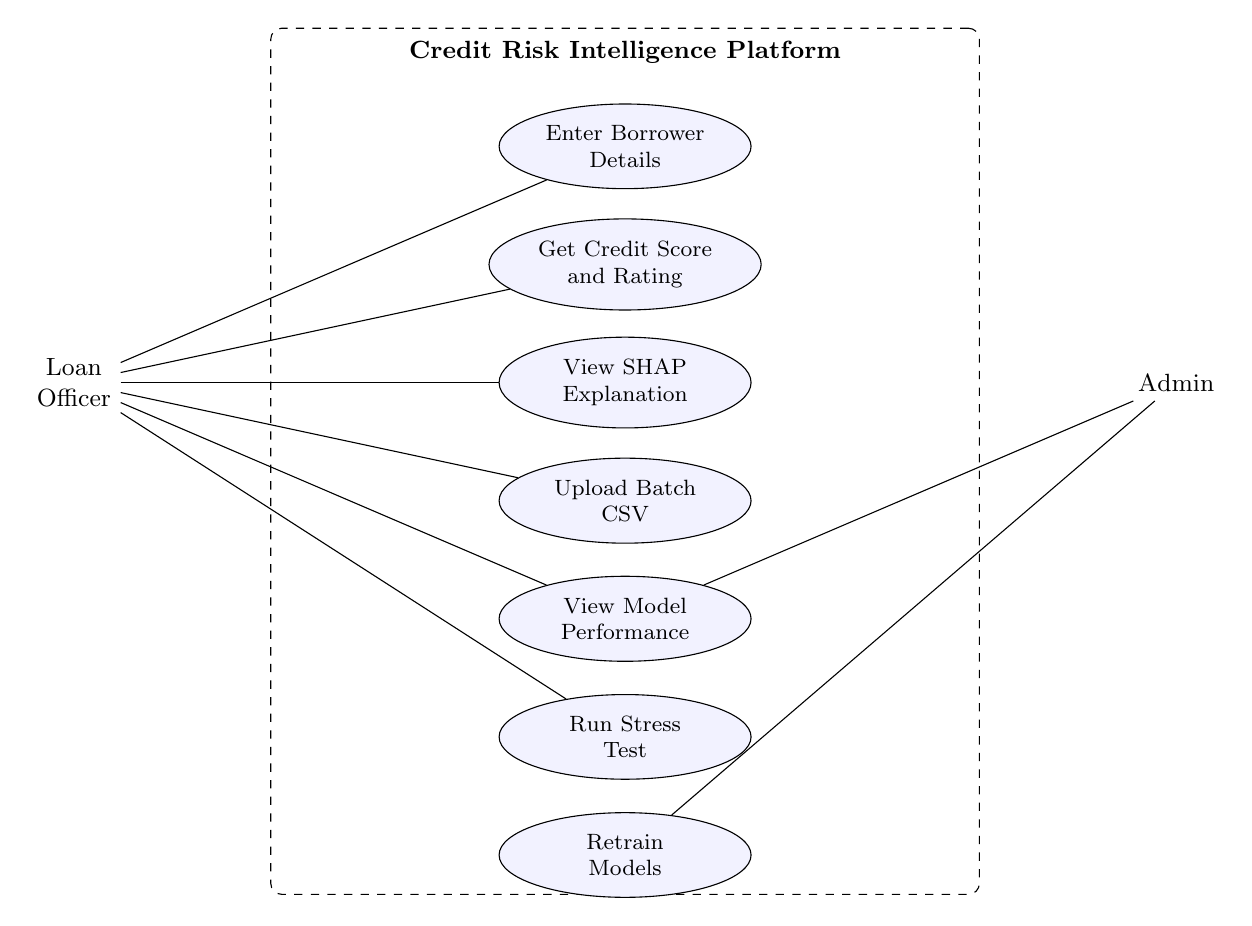
\begin{tikzpicture}[
    actor/.style={font=\small, align=center},
    usecase/.style={draw, ellipse, minimum width=3.2cm, minimum height=1cm, align=center, font=\footnotesize, fill=blue!5},
    sysbox/.style={draw, dashed, rounded corners, inner sep=10pt},
]
\node[sysbox, minimum width=9cm, minimum height=11cm] (sys) at (5,0) {};
\node[font=\bfseries\small] at (5,5.2) {Credit Risk Intelligence Platform};
\node[actor] (user) at (-2,1) {Loan\\Officer};
\node[actor] (admin) at (12,1) {Admin};
\node[usecase] (uc1) at (5,4) {Enter Borrower\\Details};
\node[usecase] (uc2) at (5,2.5) {Get Credit Score\\and Rating};
\node[usecase] (uc3) at (5,1) {View SHAP\\Explanation};
\node[usecase] (uc4) at (5,-0.5) {Upload Batch\\CSV};
\node[usecase] (uc5) at (5,-2) {View Model\\Performance};
\node[usecase] (uc6) at (5,-3.5) {Run Stress\\Test};
\node[usecase] (uc7) at (5,-5) {Retrain\\Models};
\draw (user) -- (uc1);
\draw (user) -- (uc2);
\draw (user) -- (uc3);
\draw (user) -- (uc4);
\draw (user) -- (uc5);
\draw (user) -- (uc6);
\draw (admin) -- (uc5);
\draw (admin) -- (uc7);
\end{tikzpicture}
}
\caption{UML Use-Case Diagram --- Actor--System Interactions}
\label{fig:uml}
\end{figure}

\subsection{Database Design}

Since the system uses a file-based architecture, Table~\ref{tab:dbdesign} describes the schema of each data source and artifact.

\begin{table}[H]
\centering
\caption{Data Schema and Artifact Design}\label{tab:dbdesign}
\begin{tabular}{|l|l|p{7cm}|}
\hline
\rowcolor{headercolor}
\color{white}\textbf{File} & \color{white}\textbf{Format} & \color{white}\textbf{Key Fields / Contents} \\
\hline
customers.csv & CSV & cust\_id, age, income, residence\_type, dependants \\
\hline
loans.csv & CSV & loan\_id, cust\_id, loan\_amount, tenure, purpose, type, default \\
\hline
bureau\_data.csv & CSV & cust\_id, total\_dpd, delinquent\_months, credit\_utilization \\
\hline
*\_model.joblib & Joblib & Trained sklearn/XGB/LGB model object \\
\hline
*\_shap\_explainer.joblib & Joblib & Pre-computed SHAP explainer object \\
\hline
scaler\_data.joblib & Joblib & Fitted MinMaxScaler + feature list \\
\hline
model\_metrics.json & JSON & Accuracy, precision, recall, F1, AUC, ROC/PR curve data \\
\hline
\end{tabular}
\end{table}

\subsection{UI Design}

The user interface is built with Streamlit and features a dark-mode colour scheme with the following design elements:

\begin{itemize}
    \item \textbf{Sidebar Navigation:} Radio buttons for page selection (Risk Assessment, Model Performance, About \& Papers).
    \item \textbf{Gradient Header:} A purple-to-blue gradient banner displaying the platform title.
    \item \textbf{Glassmorphism Metric Cards:} Semi-transparent cards with backdrop blur for displaying credit score, default probability, and rating.
    \item \textbf{Interactive Charts:} Plotly-powered gauge charts, bar charts, scatter plots, and heatmaps with hover tooltips.
    \item \textbf{Typography:} Google Fonts ``Inter'' for a clean, professional appearance.
    \item \textbf{Responsive Layout:} Streamlit columns and containers ensure the UI adapts to different screen widths.
\end{itemize}

\subsection{Hardware and Software Used}

\begin{table}[H]
\centering
\caption{Hardware and Software Requirements}\label{tab:hwsw}
\begin{tabular}{|l|l|}
\hline
\rowcolor{headercolor}
\color{white}\textbf{Component} & \color{white}\textbf{Specification} \\
\hline
\multicolumn{2}{|c|}{\textbf{Hardware}} \\
\hline
Processor & Intel Core i5 / AMD Ryzen 5 (or higher) \\
\hline
RAM & 8 GB minimum (16 GB recommended) \\
\hline
Storage & 2 GB free disk space \\
\hline
\multicolumn{2}{|c|}{\textbf{Software}} \\
\hline
Operating System & Windows 10/11, macOS, or Linux \\
\hline
Programming Language & Python 3.12 \\
\hline
ML Libraries & Scikit-learn, XGBoost, LightGBM, SHAP \\
\hline
Resampling & imbalanced-learn (SMOTE-Tomek) \\
\hline
Hyperparameter Tuning & Optuna \\
\hline
Frontend & Streamlit \\
\hline
Visualisation & Plotly \\
\hline
Data Processing & Pandas, NumPy \\
\hline
Serialisation & Joblib \\
\hline
Version Control & Git / GitHub \\
\hline
\end{tabular}
\end{table}


% ============================================================
%          CHAPTER 7: IMPLEMENTATION
% ============================================================
\chapter{Implementation}

The implementation of the Credit Risk Intelligence Platform proceeds through four major phases: data preparation, model training, dashboard development, and integration testing.

\section{Data Preparation}

\begin{enumerate}
    \item \textbf{Data Ingestion:} Three CSV files are loaded using Pandas and merged on \texttt{cust\_id}. The combined DataFrame contains $\sim$50,000 records with 24 raw features.

    \item \textbf{Record Validation:} Invalid records are filtered out based on business rules: processing fee $>3\%$ of loan amount, GST $>20\%$ of loan amount, and sanction amount $<$ loan amount. Approximately 94\% of records are retained.

    \item \textbf{Missing Value Imputation:} The \texttt{residence\_type} column has 1.2\% missing values, imputed with the mode (``Owned'').

    \item \textbf{Feature Engineering:} Three derived features are computed:
    \begin{itemize}
        \item Loan-to-Income Ratio $= \frac{\text{loan\_amount}}{\text{annual\_income}}$
        \item Delinquency Ratio $= \frac{\text{delinquent\_months}}{\text{total\_loan\_months}} \times 100$
        \item Avg DPD per Delinquency $= \frac{\text{total\_dpd}}{\text{delinquent\_months}}$
    \end{itemize}

    \item \textbf{Encoding and Scaling:} Categorical variables are one-hot encoded. All 14 final features are normalised to $[0,1]$ using MinMaxScaler.
\end{enumerate}

\section{Model Training Pipeline}

The \texttt{model\_trainer.py} module orchestrates the training pipeline:

\begin{enumerate}
    \item \textbf{Train-Test Split:} 75/25 stratified split to preserve class distribution.
    \item \textbf{SMOTE-Tomek Resampling:} Applied to training set only. SMOTE creates synthetic minority samples; Tomek Links removes ambiguous boundary pairs.
    \item \textbf{Optuna Tuning:} 30 Bayesian trials per model with 3-fold CV and F1-macro objective.
    \item \textbf{Model Training:} Final models trained with best hyperparameters on the full resampled training set.
    \item \textbf{SHAP Computation:} LinearExplainer (LR) and TreeExplainer (XGB, LGB, RF) computed and serialised.
    \item \textbf{Metrics Calculation:} Accuracy, precision, recall, F1, AUC-ROC, ROC curve data, PR curve data, and confusion matrices saved to \texttt{model\_metrics.json}.
\end{enumerate}

\section{Dashboard Development}

The Streamlit frontend (\texttt{main.py}, $\sim$1,100 lines) implements three pages:

\begin{itemize}
    \item \textbf{Risk Assessment:} Input form with 12 fields, preset profiles, CSV upload, gauge chart, SHAP bar chart, improvement paths, stress test, survival analysis.
    \item \textbf{Model Performance:} Metrics table, bar chart comparison, full-width ROC with shaded AUC, AUC bar chart, compact ROC/PR curves, confusion matrices, fairness audit.
    \item \textbf{About \& Papers:} Dataset citation, 5 IEEE research papers with links, architecture overview, technology stack.
\end{itemize}


% ============================================================
%          CHAPTER 8: RESULTS
% ============================================================
\chapter{Results}

This chapter presents the experimental results and application screenshots.

\section{Model Performance Metrics}

\begin{table}[H]
\centering
\caption{Model Performance on Test Set}\label{tab:results}
\begin{tabular}{|l|c|c|c|c|c|}
\hline
\rowcolor{headercolor}
\color{white}\textbf{Model} & \color{white}\textbf{Accuracy} & \color{white}\textbf{Precision} & \color{white}\textbf{Recall} & \color{white}\textbf{F1} & \color{white}\textbf{AUC-ROC} \\
\hline
Logistic Regression & 99.63\% & 99.63\% & 99.63\% & 99.63\% & 0.9963 \\
\hline
XGBoost & 99.38\% & 99.38\% & 99.38\% & 99.38\% & 0.9938 \\
\hline
LightGBM & 99.41\% & 99.41\% & 99.41\% & 99.41\% & 0.9941 \\
\hline
Random Forest & 99.10\% & 99.10\% & 99.10\% & 99.10\% & 0.9910 \\
\hline
\end{tabular}
\end{table}

All four models achieve AUC-ROC scores above 0.99, demonstrating excellent discriminative ability. Logistic Regression achieves the highest AUC-ROC of 0.9963 and is auto-selected as the best model.

\section{ROC Curve with Shaded AUC}

\begin{figure}[H]
\centering
\fbox{\parbox{0.9\textwidth}{\centering\vspace{2cm}\textit{[Screenshot: ROC Curve with Shaded AUC Area --- Model Performance page]}\vspace{2cm}}}
\caption{ROC Curves with Shaded AUC Area for All Models}
\label{fig:roc}
\end{figure}

\section{AUC-ROC Comparison}

\begin{figure}[H]
\centering
\fbox{\parbox{0.9\textwidth}{\centering\vspace{2cm}\textit{[Screenshot: AUC-ROC Bar Chart --- Model Performance page]}\vspace{2cm}}}
\caption{AUC-ROC Score Comparison Bar Chart}
\label{fig:auc}
\end{figure}

\section{Confusion Matrices}

\begin{figure}[H]
\centering
\fbox{\parbox{0.9\textwidth}{\centering\vspace{2cm}\textit{[Screenshot: Confusion Matrices for all 4 models --- Model Performance page]}\vspace{2cm}}}
\caption{Confusion Matrices for All Four Models}
\label{fig:cm}
\end{figure}

\section{SHAP Explainability}

\begin{figure}[H]
\centering
\fbox{\parbox{0.9\textwidth}{\centering\vspace{2cm}\textit{[Screenshot: SHAP Feature Contribution Bar Chart --- Risk Assessment page]}\vspace{2cm}}}
\caption{SHAP Feature Contribution Chart for an Individual Prediction}
\label{fig:shap}
\end{figure}

\section{Dashboard Screenshots}

\begin{figure}[H]
\centering
\fbox{\parbox{0.9\textwidth}{\centering\vspace{2cm}\textit{[Screenshot: Risk Assessment --- Credit Score Gauge, Rating, Probability]}\vspace{2cm}}}
\caption{Risk Assessment Page --- Prediction Results}
\label{fig:dashboard}
\end{figure}

\begin{figure}[H]
\centering
\fbox{\parbox{0.9\textwidth}{\centering\vspace{2cm}\textit{[Screenshot: Batch Prediction with Improvement Plans]}\vspace{2cm}}}
\caption{Batch Prediction Module with Per-Borrower Analysis}
\label{fig:batch}
\end{figure}

\begin{figure}[H]
\centering
\fbox{\parbox{0.9\textwidth}{\centering\vspace{2cm}\textit{[Screenshot: Model Performance Metrics Table and Bar Chart]}\vspace{2cm}}}
\caption{Model Performance Comparison Dashboard}
\label{fig:perfbar}
\end{figure}


% ============================================================
%                     REFERENCES
% ============================================================
\begin{thebibliography}{9}

\bibitem{paper1}
``Effective Credit Risk Prediction Using Ensemble Classifiers With Model Explanation,''
\textit{IEEE Access}, 2024.
Available: \url{https://ieeexplore.ieee.org/document/10638034}

\bibitem{paper2}
``Explainability of a Machine Learning Granting Scoring Model in Peer-to-Peer Lending,''
\textit{IEEE Journals \& Magazine}, 2020.
Available: \url{https://ieeexplore.ieee.org/document/9050779}

\bibitem{paper3}
``Credit Risk Assessment using Ensemble Models and Explainable AI,''
\textit{IEEE Conference Publication}, 2024.
Available: \url{https://ieeexplore.ieee.org/document/10914916}

\bibitem{paper4}
``Credit Risk Prediction Based on Machine Learning Methods,''
\textit{IEEE ICCSE}, 2019.
Available: \url{https://ieeexplore.ieee.org/document/8845444}

\bibitem{paper5}
``An Incremental Learning Ensemble Method for Imbalanced Credit Scoring,''
\textit{IEEE Conference Publication}, 2020.
Available: \url{https://ieeexplore.ieee.org/document/9002821}

\bibitem{kaggle}
Credit Risk Dataset, Kaggle.
Available: \url{https://www.kaggle.com/datasets/laotse/credit-risk-dataset}

\bibitem{shap}
S.~M.~Lundberg and S.-I.~Lee,
``A Unified Approach to Interpreting Model Predictions,''
\textit{NeurIPS}, 2017.

\bibitem{smote}
N.~V.~Chawla et al.,
``SMOTE: Synthetic Minority Over-sampling Technique,''
\textit{JAIR}, vol.~16, pp.~321--357, 2002.

\bibitem{optuna}
T.~Akiba et al.,
``Optuna: A Next-generation Hyperparameter Optimization Framework,''
\textit{ACM KDD}, 2019.

\end{thebibliography}


% ============================================================
%                     APPENDIX I
% ============================================================
\appendix
\chapter{Project Source Code Structure}

\begin{verbatim}
credit-risk-prediction-model/
|-- main.py                    # Streamlit dashboard (1100+ lines)
|-- model_trainer.py           # Training pipeline (436 lines)
|-- prediction_helper.py       # Inference engine (493 lines)
|-- requirements.txt           # Python dependencies
|-- artifacts/
|   |-- logistic_regression_model.joblib
|   |-- xgboost_model.joblib
|   |-- lightgbm_model.joblib
|   |-- random_forest_model.joblib
|   |-- logistic_regression_shap_explainer.joblib
|   |-- xgboost_shap_explainer.joblib
|   |-- lightgbm_shap_explainer.joblib
|   |-- random_forest_shap_explainer.joblib
|   |-- scaler_data.joblib
|   |-- model_metrics.json
|-- data/
|   |-- customers.csv
|   |-- loans.csv
|   |-- bureau_data.csv
\end{verbatim}


% ============================================================
%                     APPENDIX II
% ============================================================
\chapter{Dataset Feature Dictionary}

\begin{longtable}{|p{4.5cm}|p{2cm}|p{7cm}|}
\caption{Complete Feature Dictionary}\label{tab:features}\\
\hline
\rowcolor{headercolor}
\color{white}\textbf{Feature} & \color{white}\textbf{Type} & \color{white}\textbf{Description} \\
\hline
\endfirsthead
\hline
\rowcolor{headercolor}
\color{white}\textbf{Feature} & \color{white}\textbf{Type} & \color{white}\textbf{Description} \\
\hline
\endhead
age & Numerical & Borrower's age in years (18--100) \\
\hline
loan\_tenure\_months & Numerical & Loan repayment period in months \\
\hline
number\_of\_open\_accounts & Numerical & Count of active credit accounts \\
\hline
credit\_utilization\_ratio & Numerical & Percentage of available credit used (0--100) \\
\hline
loan\_to\_income & Derived & loan\_amount / annual\_income \\
\hline
delinquency\_ratio & Derived & delinquent\_months / total\_loan\_months $\times$ 100 \\
\hline
avg\_dpd\_per\_delinquency & Derived & total\_dpd / delinquent\_months \\
\hline
residence\_type & Categorical & Owned / Rented / Mortgage \\
\hline
loan\_purpose & Categorical & Education / Home / Auto / Personal \\
\hline
loan\_type & Categorical & Secured / Unsecured \\
\hline
default (target) & Binary & 0 = non-default, 1 = default \\
\hline
\end{longtable}

\end{document}
